\documentclass[11pt]{article}
\usepackage[margin=1in]{geometry}
\usepackage{amsmath,amssymb,bm,booktabs,graphicx}
\usepackage[numbers,sort&compress]{natbib}
\usepackage[colorlinks=true,allcolors=blue]{hyperref}
\newcommand{\Tr}{\operatorname{tr}}
\newcommand{\Rea}{\operatorname{Re}}
\newcommand{\ket}[1]{\lvert #1\rangle}
\newcommand{\bra}[1]{\langle #1\rvert}
\newcommand{\Ga}{\Gamma}
% Generated from component JSONs; do not hand-edit numerical entries.
\newcommand{\TransportTable}{%
\begin{table}[tbp]
\centering\small
\caption{Transport predictions at retained magnetic and hopping orders. All rows have $a=1$, $k_E=0.27$. The final column uses the leading magnetic rest energy.}\label{tab:transport}
\begin{tabular}{rrrrr}\toprule
$m$ & $t/\Delta$ & $\kappa_N$ & $\kappa_\Delta$ & $\min_k(E_\Delta-E_N)$\\
\midrule
3 & 0.462963 & 0.363741773 & 0.447657681 & -0.076577370\\
6 & 0.231481 & 0.051554688 & 0.054177060 & 0.007481348\\
12 & 0.115741 & 0.006634554 & 0.006716503 & 0.002960799\\
\bottomrule\end{tabular}
\end{table}
}
\newcommand{\CanonicalTable}{%
\begin{table}[tbp]
\centering\small
\caption{Source-connected carrier levels and vertices of the canonical total-degree-two Galerkin Hamiltonian, with $a=1$, $k_E=0.27$. Energies are in the model's common energy units.}\label{tab:canonical}
\begin{tabular}{rrrrrr}\toprule
$m$ & $E_N$ & $E_\Delta-E_N$ & $g_A$ & $Z_0$ & $D_A$\\
\midrule
3 & -0.101088537 & 0.050041335 & 1.628383677 & 0.933566905 & -0.001375714\\
1 & -0.800505119 & 0.369762206 & 1.416844275 & 0.630990796 & -0.044817278\\
0.3 & -4.874884724 & 1.819400556 & 1.050426070 & 0.267248492 & -0.209156425\\
\bottomrule\end{tabular}
\end{table}
}
\newcommand{\ResponseTable}{%
\begin{table}[tbp]
\centering\small
\caption{Local neutral inelastic axial response at $m=3$ and $t=0$. The reference is fitted to both the canonical carrier energy and elastic axial vertex; both final-isospin sectors are included. The second moment is internal to $P_2$.}\label{tab:response}
\begin{tabular}{lrrr}\toprule
Observable & Canonical $P_2$ & Matched reference & Difference\\
\midrule
$\mu_0$ & 3.459829156 & 3.452001997 & +0.227\%\\
$\mu_1$ & 0.264849804 & 0.250993569 & +5.521\%\\
$\mu_{2,P_2}$ & 0.154250462 & 0.128724750 & +19.830\%\\
$\mu_1/\mu_0$ & 0.076549966 & 0.072709566 & +5.282\%\\
\bottomrule\end{tabular}
\end{table}
}
\newcommand{\ExteriorTable}{%
\begin{table}[tbp]
\centering\small
\caption{Exact exterior action of the untruncated local $h$ on the retained $m=3$ trial state at $t=0$: positive contributions to $\|Q_2h(A-g_A)\Psi_2\|^2$. These are not spectral moments of an uncomputed full ground state.}\label{tab:exterior}
\begin{tabular}{lrr}\toprule
Channel & Norm squared & Share\\
\midrule
Three fundamental loops & 0.0001599360 & 49.465\%\\
Degree-two plus fundamental loop & 0.0001607032 & 49.702\%\\
Single $10,\overline{10}$ loop & 0.0000004933 & 0.153\%\\
Single $15,\overline{15}$ loop & 0.0000022002 & 0.680\%\\
\bottomrule\end{tabular}
\end{table}
}
\newcommand{\CompactTable}{%
\begin{table}[tbp]
\centering\small
\caption{Local compact six-quark channel versus two independent nucleons in the matched $I=0$, $T_1$, charge-one channel. Both occupied cells use the same canonical $P_2$ regulator; $a=1$, $k_E=0.27$. The leading column is $(28/3)g^2/\Omega$, not a fitted penalty.}\label{tab:compact}
\begin{tabular}{rrrrr}\toprule
$m$ & $E_6$ & $2E_N$ & $E_6-2E_N$ & Leading\\
\midrule
6 & -0.0362801071 & -0.0512144430 & 0.0149343359 & 0.0150034294\\
3 & -0.1431453284 & -0.2021770734 & 0.0590317450 & 0.0600137174\\
\bottomrule\end{tabular}
\end{table}
}
\newcommand{\RotorNRadius}{0.013810611515}
\newcommand{\RotorSixRadius}{0.026056716333}
\newcommand{\RotorNRadiusUp}{0.013811}
\newcommand{\RotorSixRadiusUp}{0.026057}
\newcommand{\RotorCompactGapDown}{0.0590317}
\newcommand{\RotorNumericalMargin}{0.0053538056}
\newcommand{\RotorConservativeMargin}{0.0053527}

\title{Chromomagnetic flux correlates baryon axial response and mobility in a projected SU(3) Hamiltonian}
\author{Anonymous}
\date{}
\begin{document}
\maketitle
\begin{abstract}
We calculate how quantum chromomagnetic dressing changes both the propagation and axial response of three-quark carriers in a specified SU(3) Hamiltonian. The geometry consists of independent three-loop bouquets joined by tree bonds; electric Casimirs, canonical holonomy multiplication, quark antisymmetry and root Gauss laws are retained. Physical one- and two-quark intermediate resolvents give a nucleon transfer correction $C_N\Omega^2=-848/25$ but a Delta correction $C_\Delta\Omega^2=248/25$, where $\Omega=4\Delta$ is the local-flux to bond-electric gap ratio. Consequently the leading curvature contrast obeys $(\kappa_\Delta-\kappa_N)/\kappa_0=(1096/25)(g/\Omega)^2=(1233/250)(5/3-g_A)=(137/25)\delta_{\rm local}/\Omega$. This is an order-$g^2t^3$ dynamical relation, not an overlap estimate of a band. Canonical two-source diagonalization then resolves information absent from the leading relation. At $m=3$, $a=1$ and $k_E=0.27$, a one-source reference matched to the carrier energy and elastic axial vertex underestimates the energy-weighted axial response by $5.52\%$ and its internal second moment by $19.83\%$. An exact energy-partition sum rule identifies the first discrepancy with a changed Pauli/electric energy balance. The next-degree exterior action adds $0.2096\%$ to the internal second moment on the retained trial state, predominantly through multi-loop flux. The results isolate a calculable cross-observable consequence of chromomagnetic dressing and a spectroscopic discriminator of its higher-flux structure within a finite projected canonical model.
The same fermionic law, with no additional compact-channel coupling, places a canonical six-quark $I=0$, $T_1$ carrier above two independent nucleons in the matched charge-one channel by $0.0149343$ at $m=6$ and $0.0590317$ at $m=3$.
Numerical evaluation of a full-rotor spectral-inclusion criterion gives a positive $\RotorConservativeMargin$ ordering margin for compatible exact local eigenlevels near the computed $m=3$ carriers, without identifying their global ground states.
\end{abstract}

\section{Introduction}
A quantum gauge-field cloud changes more than the probability of finding a bare constituent configuration. Its virtual excitations enter propagation denominators, rearrange spin--flavour currents and create inelastic channels. A useful finite-Hamiltonian calculation should therefore connect observables that cannot all be recovered from one cloud probability. Here we ask whether an axial deficit predicts a change in baryon mobility when the latter is calculated with actual electric resolvents, and which axial response remains distinguishable after elastic observables have been matched.

The ingredients have important precedents. Ordinary--hybrid baryon mixing and axial recoupling were analysed by Chow, Pirjol and Yan \cite{Chow1999HybridBaryons}; gluonic baryon excitations also have direct lattice-QCD motivation \cite{Dudek2012HybridBaryons}. Baryon hopping at third order in quark hopping, including its electric denominators, is an established strong-coupling mechanism \cite{Bringoltz2003StrongCouplingBaryons,Unger2022StrongCouplingExpansion}. Gauge-reduced Hamiltonian loop states and effective-Hamiltonian constructions are likewise established \cite{Ligterink2000HamiltonianLatticeGaugeTheory,Ligterink2001StatesEffectiveHamiltonians}. Finite canonical representation projection should not be conflated with the distinct quantum-link construction \cite{Chandrasekharan1997QuantumLinkModels}. None of those general mechanisms is the novelty asserted here.

There is also rigorous strong-coupling work beyond a bare transfer amplitude. Faria da Veiga, O'Carroll and Schor established isolated baryon dispersion curves in a one-flavour Euclidean lattice theory \cite{FariaDaVeiga2003UnderstandingBaryons}; their subsequent analysis resolved dispersion through fifth hopping order and component-dependent spectral corrections \cite{FariaDaVeiga2004BaryonSpectrum}. The earlier $2+1$-dimensional two-component formulation has no internal spin, and its two branches are baryon and antibaryon. In the later formulation, the $s=\pm3/2,\pm1/2$ labels are components of a symmetric three-quark spin-$3/2$ construction, not nucleon and Delta species. Bent hopping paths give an $18\varkappa^6+O(\varkappa^7)$ splitting between component-labelled masses in two spatial dimensions, with cancellation through sixth order in three dimensions; here $\varkappa$ denotes their hopping parameter, not our curvature. Their rigorous isolated-dispersion results are stronger global spectral statements than we establish here. Our different two-flavour Pauli--bouquet Hamiltonian instead permits the particular nucleon--Delta curvature/axial comparison and elastic-matched inelastic discriminator derived below; no parameter identification or numerical disagreement between the two theories is implied. Its dilute single-baryon, empty-background transport does not address finite-density composite-baryon statistics.

Quark-based hadron mass relations \cite{DeRujula1975HadronMasses} and short-range interactions between non-strange baryons \cite{Oka1981ShortRangeBaryonInteraction} also provide established context for the compact-channel comparison below. Our additional calculation keeps the canonical rotor field explicit and its coupling unchanged across three- and six-quark occupancies.

Our contribution is the explicit coefficient and cross-observable relation obtained when chromomagnetic insertions are propagated through the physical transfer resolvents, followed by a canonical higher-flux response calculation. Endpoint dressing alone would predict mobility changes proportional to a compact-source Casimir. The actual intermediate contractions contain additional terms and give opposite-sign nucleon and Delta corrections. The resulting curvature contrast shares its microscopic coupling with the axial deficit and local splitting. At the next level, canonical two-source states invalidate a probability-only elastic relation and produce a sizable inelastic difference even after matching the energy and elastic vertex. We derive an energy-partition interpretation rather than treating that difference as an unexplained numerical residual.

The calculation is a nonrelativistic lattice model with specified quark, orbital and Pauli operators, not a derivation of continuum QCD. The terms nucleon and Delta label vacuum-connected isospin and cubic-symmetry carrier branches. We first specify the common Hamiltonian and its order-specific source reduction, then derive transport, and finally examine finite canonical axial response and its exterior.

\section{Canonical bouquet--tree Hamiltonian}
\subsection{Geometry, operators and electric costs}
At each matter site $s$ attach three independent oriented four-edge loops, labelled $k=x,y,z$, sharing only their root. Connect neighbouring roots by tree bonds. A loop holonomy $U_{sk}\in SU(3)$ transforms by conjugation at the root. Eliminating the three nonroot gauge transformations of each isolated loop leaves the electric operator $4k_E C_{2,sk}$: all four edges carry the same representation. The loops do not share edges; thus the electric cross derivatives appropriate to shared-edge plaquettes are not part of this geometry.

There are twelve CAR modes per root, $(u,d)\otimes(\uparrow,\downarrow)\otimes\mathbf3$. With $\Tr(T^aT^b)=\delta^{ab}/2$, define
\begin{align}
 b_{sk}^a&=i\Tr[T^a(U_{sk}-U_{sk}^\dagger)], &
 G_{ak,s}&=c_s^\dagger(1_f\otimes\sigma_k\otimes T^a)c_s,\\
 H_{\rm loc,s}&=4k_E\sum_k C_{2,sk}+c_P\sum_{ak}b_{sk}^aG_{ak,s}, &
 c_P&=-\frac{1}{2ma^2}. \label{eq:local}
\end{align}
If $B^a_k=b^a_k/(qa^2)$ is used as the magnetic field convention, the Pauli coefficient $-q/(2m)$ gives precisely $c_P$; the gauge charge cancels. This is the adopted effective Pauli interaction, not an exact identity for a finite-difference Dirac operator.

For a directed tree bond $x\to y$ with canonical holonomy $U_{yx}$, the Hamiltonian is
\begin{align}
 H&=\sum_s H_{\rm loc,s}+k_E\sum_{\ell\in\mathrm{tree}}C_{2,\ell}
       +\sum_{\langle xy\rangle}(T_{yx}+T_{yx}^\dagger),\\
 T_{yx}(A)&=-t\sum_{f,\sigma,a,b}c^\dagger_{y,f\sigma a}(U_{yx})_{ab}
                  c_{x,f\sigma b}e^{-iq_f A},\\
 t&=\frac{1}{2ma^2},\qquad q_u=\frac23,\quad q_d=-\frac13. \label{eq:tree}
\end{align}
The phase $A$ denotes the dimensionless uniform electromagnetic line integral on that bond. Common quark rest energy and the on-site kinetic discretization constant are omitted from energy differences. No occupancy-dependent selector gap is added. Both roots obey Gauss law, including matter, bouquet-conjugation charge and the appropriate left or right bond-electric charge. Intermediate occupancies $(N_x,N_y)=(2,1),(1,2)$ are genuine CAR sectors, not replaced by compact three-quark overlaps.

A fundamental tree excitation costs $\Delta=4k_E/3$. The first loop excitation costs
\begin{equation}
 \Omega=\frac{16k_E}{3}=4\Delta,\qquad
 g=\frac{c_P}{\sqrt3}=-\frac{1}{2\sqrt3ma^2}. \label{eq:matching}
\end{equation}
We use $\hbar=1$ and a common model energy unit; the numerical examples set $a=1$. A curvature has units energy times length squared.

\subsection{Canonical multiplication and finite Hilbert spaces}
The normalized Peter--Weyl states are $\ket{r,m,n}=\sqrt{d_r}D^r_{mn}(U)$. For an isometric Clebsch--Gordan intertwiner $C: s\to\mathbf3\otimes r$, canonical multiplication is
\begin{equation}
 \bra{s,M,N}U_{ab}\ket{r,m,n}
 =\sqrt{\frac{d_r}{d_s}}\,C^M_{am}C^{N*}_{bn}. \label{eq:PW}
\end{equation}
All retained-to-retained blocks, including the epsilon-tensor $\mathbf3\to\overline{\mathbf3}$ block, are included before diagonalization. The local conjugation generator on wavefunction coefficients is the sum of the left and right actions in the implemented convention; it obeys $[Q_c,b_a]=if_{cab}b_b$.

We distinguish three spaces. The source-only field is vacuum plus the 24 normalized states $\ket{ak}=\sqrt3 b_k^a\ket0$, hence dimension 25. The PW19 loop retains $\mathbf1,\mathbf3,\overline{\mathbf3}$ and its full three-loop product has $19^3=6859$ states. The canonical two-source calculation additionally retains $\mathbf6,\overline{\mathbf6},\mathbf8$ on each loop, whose local Peter--Weyl dimension is 155, and restricts the sum of the minimal representation degrees to two. Its field dimension is
\begin{equation}
 \dim P_2=1+3(18)+3(136)+3(18^2)=1435. \label{eq:dimension}
\end{equation}
This contains every $bb\ket0$ channel: $\mathbf3\otimes\mathbf3=\mathbf6+\overline{\mathbf3}$, $\mathbf3\otimes\overline{\mathbf3}=\mathbf1+\mathbf8$, their conjugates and products on distinct loops. The true electric costs are used, including $C_2(6)=10/3$ and $C_2(8)=3$. For the nonlinear local calculation we isolate one bouquet, set spatial hopping to zero and define
\begin{equation}
 h\equiv H_{{\rm loc},s}=h_E+V,\qquad h_2=P_2hP_2,\qquad
 h_E=4k_E\sum_k C_{2,sk}.
 \label{eq:localprojection}
\end{equation}
Here $h$ acts at fixed local quark number: three for the axial carrier calculation and six for the compact-channel comparison below. All nonlinear carrier energies, elastic vertices and axial moments refer to the corresponding $h_2$; it is not a projection of the spatial hopping Hamiltonian $H$. Its retained representation channels suffice for fourth-order local vacuum-return perturbation theory. Its nonlinear eigenvalues are exact for the declared Galerkin projection, not for a terminated canonical tower. Thus the transport expansion and the nonlinear local observables are different consumers of the specified bouquet--tree law, not a solved finite-hopping joined spectrum.
The shorthand $t=0$ denotes zeroth order in intercell hopping, with the local $m,k_E$ and Pauli coefficients held fixed. Equivalently, an auxiliary multiplier $\zeta$ of the spatial hopping term is set to zero; this does not change the common-mass matching $g=-t_{\rm NR}/\sqrt3$ when the physical spatial coefficients are combined.

\subsection{Why the transport source reduction is exact at its order}
Haar orthogonality gives
\begin{equation}
 \bra0 b_k^a b_l^b\ket0=\frac13\delta^{ab}\delta_{kl},\qquad
 H_E\ket{ak}=\Omega\ket{ak}. \label{eq:gram}
\end{equation}
Holonomy inversion $J_k:U_k\mapsto U_k^\dagger$ preserves Haar measure and electric energy and makes $b_k^a$ odd. Every magnetic source is odd, so
\begin{equation}
 P_{\rm src}b_k^aP_{\rm src}=0. \label{eq:odd}
\end{equation}
The full degree-one field space is 54-dimensional, not 24-dimensional, and its magnetic block is nonzero: it includes even combinations orthogonal to the odd sources. Nevertheless a vacuum-return word with only two total magnetic insertions can visit only vacuum, one source and vacuum. Tree hopping does not act on the bouquet variables. Equations~\eqref{eq:gram}--\eqref{eq:odd} therefore embed the source calculation exactly in the canonical Hamiltonian through $g^2t^3$. Extra canonical channels first enter vacuum-return transport at $g^4$; no nonlinear equivalence to the 25-state model follows.

\subsection{Carrier identity and current}
The compact seeds are colour singlets with three quarks in one local orbital. Their spin--isospin labels are $S=I=1/2$ and $S=I=3/2$, chosen at $I_3=S_z=1/2$. Both charged seeds have $Q=1$; the neutron follows by isospin. Fixing $I_3=1/2$ and projecting exact isospin leaves 70 matter states for $I=1/2$ and 20 for $I=3/2$. Fermionic signs are retained throughout.

The bouquet has proper cubic symmetry, not continuous spatial $SO(3)$. Signed loop permutations are accompanied by holonomy inversion for a reversed axial direction and the actual quark-spin rotation. The source-connected states carry a closed binary-cubic $\Ga_6$ doublet and $\Ga_8$ quartet, respectively. At the canonical $m=3$ input their rotation characters are $(\chi(C_3),\chi(C_4))=(1,\sqrt2)$ and $(-1,0)$; orbit closure residuals are below $7.7\times10^{-15}$ and $6.5\times10^{-14}$. We use $N$ and $\Delta$ as these branch labels, not as a claim of exact continuous-spin multiplets. The eigensolver follows the vacuum-connected branches; it does not establish a global lowest state against every orthogonal branch or cubic irrep.

The neutral axial operator and elastic vertex are
\begin{equation}
 A=c^\dagger(\tau_3\otimes\sigma_z\otimes1_c)c,\qquad
 g_A=\bra{\Psi_N}A\ket{\Psi_N}. \label{eq:axial}
\end{equation}
This specified one-body spin--flavour current is not a matched continuum axial current or a chiral-sea construction.

\section{Transport from physical electric resolvents}
\subsection{Endpoint and denominator expansion}
On a compact colour-singlet seed, the source algebra gives
\begin{equation}
 \sum_{ak}G_{ak}^2\ket B=\lambda_B\ket B,\qquad
 \lambda_N=16,\quad\lambda_\Delta=8.
\end{equation}
One can obtain these eigenvalues directly before building the field space. For three quarks,
\begin{equation}
 \sum_{ak}G_{ak}^2=12+2\sum_{i<j}
   (\bm\sigma_i\cdot\bm\sigma_j)(\bm T_i\cdot\bm T_j).
\end{equation}
On the colour singlet each pair has $\bm T_i\cdot\bm T_j=-2/3$, while
$\sum_{i<j}\bm\sigma_i\cdot\bm\sigma_j=2S(S+1)-9/2$.
Thus $\lambda_S=18-(8/3)S(S+1)$, giving the two values above. The constant 12 is the three-quark one-body contribution, since a single quark obeys $\sum_{ak}(\sigma_kT^a)^2=4$.
The cyclic source-only problem has $E_B=(\Omega-\sqrt{\Omega^2+4\lambda_Bg^2})/2$. Its order-consistent endpoint expansion, also the canonical expansion to the order used here, is
\begin{align}
 \ket{\widetilde B}&=\left(1-\frac{\lambda_Bg^2}{2\Omega^2}\right)\ket{B,0}
       -\frac g\Omega\sum_{ak}\ket{ak}G_{ak}\ket B+O(g^2)_{\perp}+O(g^3)_{\rm src},\\
 E_B&=-\frac{\lambda_Bg^2}{\Omega}+O(g^4). \label{eq:endpoint}
\end{align}
The canonical $O(g^2)_{\perp}$ amplitude does not contribute to a vacuum-return transfer with two insertions: the other endpoint or a further insertion would have to close its nonvacuum field. Normalization and first-source terms do contribute.

Let $D=\Delta+\Omega n_{\rm src}$ on the two intermediate matter sectors, and let $V$ be the sum of the two local source vertices with $g$ stripped off. Expanding at the compact source energy gives
\begin{equation}
 R_B=(E_B-H_{\rm int})^{-1}
 =-D^{-1}+gD^{-1}VD^{-1}
 +g^2\left[\frac{\lambda_B}{\Omega}D^{-2}
                 -D^{-1}VD^{-1}VD^{-1}\right]+O(g^3). \label{eq:resolvent}
\end{equation}
The positive energy-shift term follows because $E_B=-\lambda_Bg^2/\Omega$; omitting it would change the answer. The denominators are $\Delta$ and $L=\Delta+\Omega$, not an adjustable baryon gap.

\subsection{Contractions and transfer coefficient}
We evaluate $\bra{\widetilde B_y}T R_B T R_B T\ket{\widetilde B_x}$ with the physical one- and two-quark CAR states. The bare colour-singlet transfer is $M_0=-6t^3/\Delta^2$. Useful elementary identities are
\begin{align}
 \{c_i,c_j^\dagger\}&=\delta_{ij},\quad
 \sum_aT^a_{ij}T^a_{kl}=\tfrac12(\delta_{il}\delta_{jk}-\tfrac13\delta_{ij}\delta_{kl}),\\
 \sum_k(\sigma_k)_{\alpha\beta}(\sigma_k)_{\gamma\delta}
 &=2\delta_{\alpha\delta}\delta_{\beta\gamma}-\delta_{\alpha\beta}\delta_{\gamma\delta},\\
 \int dU\,U_{a_1b_1}U_{a_2b_2}U_{a_3b_3}
 &=\frac16\epsilon_{a_1a_2a_3}\epsilon_{b_1b_2b_3}. \label{eq:contraction-identities}
\end{align}
The contractions can be reduced analytically by labelling quarks $1,2,3$ in their order of departure. Define $q_i^{ak}=\sigma_{k,i}T_i^a$, with a dot denoting the sum over $a,k$, and $\bm{\mathcal Q}=\bm q_1+\bm q_2+\bm q_3$. Each quark has $\bm q_i^2=4$ and the compact source has $\bm{\mathcal Q}^2=\lambda$. The six bare transfer orderings carry equal normalized weight: the CAR permutation signs and the Haar epsilon contraction in Eq.~\eqref{eq:contraction-identities} combine into the same colour-singlet transfer amplitude. Thus the ordering-averaged distinct-pair contraction is
\begin{equation}
 \overline{\bm q_i\cdot\bm q_j}=\frac{\lambda-12}{6},\qquad i\ne j.
\end{equation}
The two intermediate occupancies have root vertices $(\bm q_2+\bm q_3,\bm q_1)$ and $(\bm q_3,\bm q_1+\bm q_2)$. Consequently the same-resolvent, cross-resolvent, adjacent-endpoint and far-endpoint factors, respectively, are
\begin{align}
 \overline{(\bm q_2+\bm q_3)^2+\bm q_1^2}
 &=12+\frac{\lambda-12}{3}=8+\frac{\lambda}{3},\\
 \overline{\bm q_3\cdot(\bm q_2+\bm q_3)+(\bm q_1+\bm q_2)\cdot\bm q_1}
 &=8+\frac{\lambda-12}{3}=4+\frac{\lambda}{3},\\
 \overline{\bm{\mathcal Q}\cdot(\bm q_2+\bm q_3)}
 &=8+\frac{2(\lambda-12)}{3}=\frac{2\lambda}{3},\\
 \overline{\bm{\mathcal Q}\cdot\bm q_3}
 &=4+\frac{\lambda-12}{3}=\frac{\lambda}{3}.
 \label{eq:orderedcontractions}
\end{align}
These identities retain the one-body pieces as well as the pair contractions and give the following normalized insertion factors:
\begin{center}
\begin{tabular}{lr}
\toprule
Insertion contraction & Dimensionless factor\\\midrule
Two vertices in the same resolvent & $8+\lambda/3$\\
One vertex in each resolvent & $4+\lambda/3$\\
Adjacent endpoint--vertex & $2\lambda/3$\\
Far endpoint--vertex & $\lambda/3$\\\bottomrule
\end{tabular}
\end{center}
For $N$ these are $40/3,28/3,32/3,16/3$; for $\Delta$ they are $32/3,20/3,16/3,8/3$. In particular the constants 8 and 4 are not an endpoint-overlap factor. Summing the normalization, source-energy, same-resolvent, cross-resolvent and the two endpoint--vertex classes gives
\begin{align}
 M_B&=-\frac{6t^3}{\Delta^2}(1+C_{\lambda_B}g^2)+O(g^4t^3)\quad\text{at third hopping order},\\
 C_\lambda&=-\frac{\lambda}{\Omega^2}-\frac{2\lambda}{\Omega\Delta}
 +\frac{2(8+\lambda/3)}{\Delta L}+\frac{4+\lambda/3}{L^2}\notag\\
 &\quad+\frac{4\lambda}{3\Omega L}+\frac{2\lambda\Delta}{3\Omega L^2}. \label{eq:C}
\end{align}
The first two terms come from endpoint normalization and the carrier energy in the two resolvents. The following two terms retain respectively the single- and double-resolvent magnetic insertions. The final two are the adjacent and far endpoint terms. Endpoint excitation on both sides, with no intermediate magnetic insertion, vanishes because the fields belong to independent roots.

For $r=\Omega/\Delta$,
\begin{equation}
 C_\lambda\Omega^2=
 \frac{48r^3+60r^2-\lambda(4r^3+8r^2+6r+3)}{3(r+1)^2}.
\end{equation}
At the canonical ratio $r=4$ this is $(1344-137\lambda)/25$, and hence
\begin{equation}
 C_N\Omega^2=-\frac{848}{25},\qquad
 C_\Delta\Omega^2=\frac{248}{25}. \label{eq:coefficients}
\end{equation}
The universal intermediate contribution permits the Delta's positive mobility shift, but cancels from the difference $C_\Delta-C_N$. The contrast comes from the full $\lambda$-dependent denominator and mixed-endpoint structure, not from the universal term alone. An endpoint-only estimate would instead give a contrast $8(g/\Omega)^2$ rather than $1096(g/\Omega)^2/25$.

The tree-link representations $\mathbf1,\mathbf3,\overline{\mathbf3}$ suffice for this coefficient: after two forward hops a sextet cannot combine with the third fundamental to end in a singlet; local bouquet vertices do not change the bond representation. Both independent one-source root sectors are included. Two simultaneously excited roots cannot close a vacuum-return path with only two magnetic insertions.

\subsection{Curvature, axial response and local splitting}
The same resolvents give the return energy per empty neighbour,
\begin{equation}
 \Sigma_B^{\rm bond}=-\frac{3t^2}{\Delta}(1+D_{\lambda_B}g^2),\qquad
 D_\lambda\Omega^2=-\frac{2r[\lambda(r+1)-12r]}{3(r+1)}. \label{eq:return}
\end{equation}
For a dilute one-dimensional nearest-neighbour embedding,
\begin{equation}
 E_B(k)=-\frac{\lambda_Bg^2}{\Omega}+2\Sigma_B^{\rm bond}+2M_B\cos(ka),\quad
 \kappa_B=\partial_k^2E_B(0)=-2a^2M_B,\quad
 \kappa_0=\frac{12t^3a^2}{\Delta^2}. \label{eq:band}
\end{equation}
This is an analytical effective dispersion at the stated orders. It is not deduced from the zero-field probability $Z_0$.

The compact source current has $\bra N A\ket N=5/3$ and normalized first-source expectation $10/9$. Thus its leading axial deficit and local splitting are
\begin{equation}
 \frac53-g_A=\frac{80}{9}x+O(x^2),\qquad
 \delta_{\rm local}=E_\Delta-E_N=8\Omega x+O(\Omega x^2),\qquad x=\frac{g^2}{\Omega^2}. \label{eq:leadinglocal}
\end{equation}
Combining Eqs.~\eqref{eq:coefficients}--\eqref{eq:leadinglocal} gives the principal result,
\begin{equation}
 \boxed{\frac{\kappa_\Delta-\kappa_N}{\kappa_0}
 =\frac{1096}{25}\left(\frac g\Omega\right)^2
 =\frac{1233}{250}\left(\frac53-g_A\right)
 =\frac{137}{25}\frac{\delta_{\rm local}}{\Omega}.} \label{eq:principal}
\end{equation}
All equalities retain the leading magnetic order and third hopping order. Corrections to the normalized contrast include $O(x^2)$ and $O(x\eta^2)$, where $\eta=t/\Delta$. The $g_A$ and $\delta_{\rm local}$ in this relation are their order-consistent leading values, not the nonlinear canonical values below.

Under the microscopic matching $g=-t/\sqrt3$, $x=\eta^2/48$, so
\begin{equation}
 \begin{aligned}
 \frac{\kappa_N}{\kappa_0}&=1-\frac{53}{75}\eta^2,\qquad
 &\frac{\kappa_\Delta}{\kappa_0}&=1+\frac{31}{150}\eta^2,\\
 \frac{\kappa_\Delta-\kappa_N}{\kappa_0}&=\frac{137}{150}\eta^2,\qquad
 &\frac53-g_A&=\frac5{27}\eta^2.
 \end{aligned}\label{eq:eta}
\end{equation}
At $g=0$ the electric and quark-hopping Hamiltonian is spin--flavour $SU(4)$ invariant. The compact colour-singlet three-quark states form its symmetric 20-dimensional multiplet, containing the four nucleon and sixteen Delta spin--isospin states. Consequently pure-$g^0$ hopping corrections are common to these branches. Bare higher-hopping terms can change the absolute curvatures at the same matched heavy-mass order as the displayed magnetic correction, but cancel from the contrast. In the matched counting the leading contrast is of order $\eta^5$ in units $\Delta a^2$; $g^4t^3$ and $g^2t^5$ begin at order $\eta^7$. This does not supply missing relativistic/Foldy--Wouthuysen operators or a complete Dirac $1/m$ expansion.

The corresponding momentum-dependent splitting at the retained orders is
\begin{equation}
 E_\Delta(k)-E_N(k)=\delta_{\rm local}
 \left[1-4\eta^2-\frac{411}{25}\eta^3\cos(ka)\right]. \label{eq:momentumgap}
\end{equation}
Unlike the curvature contrast, its constant part is sensitive to omitted $g^4$ rest energies. The same one-body magnetic operator gives $\mu_p=3g_A/(10m)$ and $\mu_n=-g_A/(5m)$ at this order; these recoupling relations are supplementary, whereas Eq.~\eqref{eq:principal} requires the dynamical transfer calculation.

\TransportTable
\begin{figure}[tbp]\centering
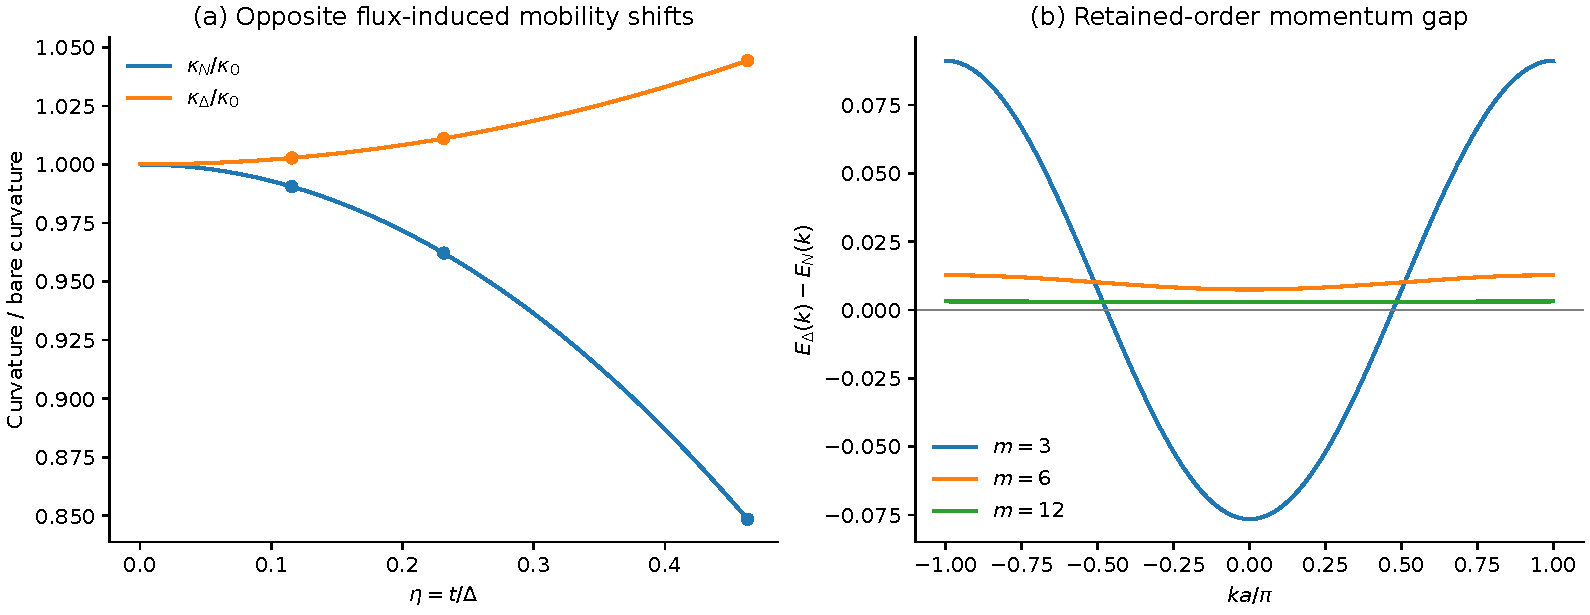
\includegraphics[page=1,width=\textwidth]{journal_flux_axial_mobility_figures_20261019.pdf}
\caption{Analytical retained-order transport predictions and source-derived numerical coefficients. (a) Opposite normalized curvature corrections; points are the executed mass rows, while lines use Eq.~\eqref{eq:eta}. Only the contrast is protected against common bare higher-hopping terms. (b) Eq.~\eqref{eq:momentumgap}, retaining its adverse $m=3$ crossing rather than replacing it by a claimed stable band.}\label{fig:transport}
\end{figure}

At $m=6$, $a=1$, $k_E=0.27$, one has $\eta=0.231481$ and $\kappa_\Delta-\kappa_N=0.0026223721$. The leading-rest gap minimum is $0.0074813482$. Replacing only the rest energy by the exact 25-state source-only energy changes the minimum to $0.0071505090$; that is a partial finite-cell resummation, not a canonical higher-order band. The $m=3$ row has $\eta=0.462963$ and a crossing in the truncated dispersion. Positive local denominators do not by themselves guarantee finite-hopping band ordering.

For completeness, the one-quark mixed Casimir is 4 and the two-quark spectrum is $6,20/3,26/3,12$. Within the source-only finite cell, the unrestricted threshold is bounded below by $\Delta+E(4)+E(12)$, where $E(\lambda)$ is the cyclic energy above. Gauss projection can only raise this bound. Its margin above the compact nucleon at $m=6$ is $0.3598364867$. This is a local finite-cell threshold statement; it is not a bound on the untruncated canonical spatial spectrum.

\section{Canonical two-source axial structure}
\subsection{A coherence law beyond the vacuum probability}
We now diagonalize the isolated-bouquet $h_2$ of Eq.~\eqref{eq:localprojection} at $t=0$, without expanding $g$. This is a different approximation to the same local canonical law, not a nonlinear completion of the calculated band. The energies, vertices and moments in this section are local observables. Let $v$ be the compact vacuum seed, $s$ its normalized magnetic source, and write the source-connected carrier as
\begin{equation}
 \ket\Psi=\alpha\ket v+\beta\ket s+\ket\chi,\qquad
 Z_0=|\alpha|^2,\quad W_1=|\beta|^2,\quad r_\chi=\|\chi\|^2=1-Z_0-W_1.
\end{equation}
Here $\chi$ is orthogonal to both $v$ and $s$; it is not synonymous with total representation degree two. Since $A$ preserves field degree, its vacuum--excluded matrix element vanishes for the selected seed. The exact finite-space decomposition is
\begin{align}
 g_A&=\frac53 Z_0+\frac{10}{9}W_1+\bra\chi A\ket\chi
            +2\Rea\{\beta^*\bra s A\ket\chi\},\\
 D_A&\equiv g_A-\left(\frac{10}{9}+\frac59 Z_0\right)
 =\bra\chi(A-10/9)\ket\chi+2\Rea\{\beta^*\bra s A\ket\chi\}. \label{eq:defect}
\end{align}
In the 25-state cyclic reference, $r_\chi=0$ and the straight line is exact: $g_A=5/3-(5/9)\rho$, where $\rho=1-Z_0$. Canonical multiplication populates additional channels and coherences. Equation~\eqref{eq:defect}, rather than a replacement fitted straight line, explains the deviation. The conservative bound $\|A\|\leq3$ implies $|D_A|\leq(37/9)r_\chi+6\sqrt{W_1r_\chi}$.

\CanonicalTable
At $m=3$, the canonical carrier has $r_\chi=0.00203796248$ and
\begin{equation}
 D_A=0.00102274393-\frac{10}{9}(0.00203796248)-0.00013405545
 =-0.00137571428.
\end{equation}
The three terms are the excluded axial expectation, its subtracted one-source baseline and the included--excluded coherence. The conditional axial vertices at zero, one and two active loops are $5/3$, $1.1001135961$ and $0.5718418794$. Even the one-active-loop layer is no longer a single source vector. Colour-decuplet matter has probability $0.00051865583$, and cross-quark-spin axial terms contribute $0.05760776625$; diagonal colour/spin probabilities alone do not reconstruct the current.

The full PW19 bouquet at this mass gives $g_A=1.6285999982$, $Z_0=0.9338714818$ and $D_A=-0.0013286027$. Restoring the canonical local $6,\overline6,8$ channels changes but does not remove the effect. This comparison is evidence of the mechanism's persistence under a material representation change, not a bound on canonical cutoff error. Smaller masses in Table~\ref{tab:canonical} are interaction stress regimes, not controlled continuum or heavy-particle predictions.

\subsection{Matched-energy, matched-vertex inelastic response}
For the stationary carrier eigenstate define $y=(A-g_A)\Psi$ and
\begin{equation}
 S_A(\omega)=\sum_{\nu\ne\Psi}|\bra\nu A\ket\Psi|^2
           \delta(\omega-E_\nu+E),\qquad
 \mu_j=\bra y(h_2-E)^j\ket y,\quad j=0,1,2. \label{eq:moments}
\end{equation}
The final-state sum is complete at fixed $I_3=1/2$ and includes both $I=1/2$ and $I=3/2$ via the full CAR current. Since the initial state is a source-connected eigenstate rather than a proved global ground state, $\omega$ need not be globally positive; $\mu_1$ is the signed energy-weighted moment of that stationary-state response. $\mu_0$ and $\mu_2$ remain nonnegative. No individual inelastic poles are inferred from these moments.

To distinguish higher-flux information from simple elastic refitting, choose a positive-gap 25-state reference with the same $E$ and $g_A$. Its necessary source weight and parameters are
\begin{equation}
 p=\frac95\left(\frac53-g_A\right),\qquad
 \Omega_{\rm fit}=-\frac{E(1-2p)}p,\qquad
 g_{\rm fit}^2=\frac{E^2(1-p)}{16p}. \label{eq:fit}
\end{equation}
For a negative-energy lower cyclic state with positive gap, $0<p<1/2$. At $m=3$, $\Omega_{\rm fit}=1.2648008013$, $|g_{\rm fit}|=0.0928963651$, and the reference eigen-residual is $1.56\times10^{-16}$. Its full current includes both final-isospin sectors, exactly as the canonical response does.

\ResponseTable
The inelastic differences in Table~\ref{tab:response} survive matching both elastic observables. The $\mu_0$ difference measures changed two-quark axial correlations because $\mu_0=\langle A^2\rangle-g_A^2$. The $5.52\%$ first-moment and $19.83\%$ second-moment excesses are more discriminating than the $0.227\%$ integrated-strength difference. At this mass the $I=3/2$ final sector supplies $3.4076417047$ of the total strength, while $I=1/2$ supplies $0.0521874514$. Projecting the current back into the initial isospin would omit most of this response. Bare $N$--$\Delta$ degeneracy makes an order-one integrated strength compatible with small energy-weighted moments; it is not evidence of a large high-energy rate.

At $m=1$ the internal second moments are $2.2581575336$ and $0.9191254341$ in the canonical and fitted-reference calculations. At $m=0.3$, the required $p=1.10923307$ does not permit this positive-gap reference. We report that failure rather than supplying an unphysical negative-gap fit.

\begin{figure}[tbp]\centering
\includegraphics[page=2,width=\textwidth]{journal_flux_axial_mobility_figures_20261019.pdf}
\caption{Canonical axial structure. (a) The source-connected degree-two carrier vertices depart from the probability-only line of the vacuum/one-source reference. The line is the declared analytical relation, not a fit to the canonical points. (b) At $m=3$, energy- and vertex-matched references still differ in the three neutral-current moments. The plotted second moment is internal to $P_2$.}\label{fig:response}
\end{figure}

\subsection{Energy partition explains the first-moment excess}
Write $V_k=c_P\sum_a b_k^aG_{ak}$ and $F_{ak}=c^\dagger(\tau_3\otimes\sigma_k\otimes T^a)c$. The CAR one-body commutator identity $[c^\dagger Mc,c^\dagger Nc]=c^\dagger[M,N]c$ gives
\begin{align}
 [h_2,A]&=2ic_P\sum_a(b_y^aF_{ax}-b_x^aF_{ay}),\\
 \mu_1&=\frac12\langle[A,[h_2,A]]\rangle=-2\langle V_x+V_y\rangle, \label{eq:sumrule}\\
 \mu_{2,P_2}&=\|[h_2,A]\Psi\|^2
 =4c_P^2\left\langle\left[\sum_a(b_y^aF_{ax}-b_x^aF_{ay})\right]^2\right\rangle_{P_2}. \label{eq:secondcomm}
\end{align}
All magnetic products in Eq.~\eqref{eq:secondcomm} are projected operator products of the local $h_2$. They should not be replaced by unprojected products when interpreting its internal second moment.

The diagonal anisotropy among $V_x,V_y,V_z$ transforms as the cubic $E$ irrep. The carrier doublet obeys $\Ga_6^*\otimes\Ga_6=A_1+T_1$, so it has no such diagonal matrix element. Thus $\langle V_x\rangle=\langle V_y\rangle=\langle V_z\rangle$ and
\begin{equation}
 \boxed{\mu_1=-\frac43\langle V\rangle,\qquad
 \langle h_E\rangle=E+\frac34\mu_1,\qquad V=V_x+V_y+V_z.} \label{eq:partition}
\end{equation}
This follows from the actual cubic irrep, without assigning a continuous $J^2$. The moments were calculated by direct Hamiltonian action; Eq.~\eqref{eq:partition} is an independent algebraic interpretation, not a separate measured isotropy diagnostic.

At $m=3$, Eq.~\eqref{eq:partition} gives $\langle V\rangle=-0.1986373533$ and $\langle h_E\rangle=0.0975488165$. The matched reference has $\langle V\rangle=-0.1882451765$ and $\langle h_E\rangle=0.0871566398$. Equal local total energy therefore conceals an extra $0.0103921767$ of electric energy compensated by greater Pauli binding. An energy-weighted axial probe together with the local carrier energy can thus reconstruct electric/Pauli energy sharing without a direct field-energy readout. This extraction uses the local $t=0$ law $h=h_E+V$; a spatial finite-hopping total energy would also require separating its kinetic contribution. The second moment additionally resolves repeated flux--quark axial correlations, accounting for its larger discrimination.

\section{Higher-flux exterior action}
The degree-two response is exact for the local $h_2$, but not automatically for the untruncated canonical local operator $h$ of Eq.~\eqref{eq:localprojection}. Spatial hopping remains zero in this section. Because $A$ preserves field representation degree, $y\in P_2$. Orthogonal decomposition gives the exact identity on this retained trial state,
\begin{equation}
 \|(h-E)y\|^2=\|P_2(h-E)y\|^2+\|Q_2hy\|^2
 =\mu_{2,P_2}+\epsilon_A,\qquad Q_2=1-P_2. \label{eq:exterior}
\end{equation}
Every output of one canonical magnetic action on $P_2$ is captured by extending the operator map to $10,\overline{10},15,\overline{15}$ and mixed-loop degree-three states. Both $U_{\rm out,in}$ and $U_{\rm in,out}$ are needed to form $b=i\Tr[T(U-U^\dagger)]$. This is an exterior action, not a degree-three diagonalization.

\ExteriorTable
At $m=3$, $\epsilon_A=0.0003233326810$, or $0.2096\%$ of the internal moment, and $\|(h-E)y\|^2=0.1545737942219$. The first two channels in Table~\ref{tab:exterior} contribute $99.17\%$: the missing response is primarily extra multi-loop flux rather than a single high-colour loop. Their bare electric costs are 4.32 for three fundamental loops, and 4.68 or 5.04 for an octet or sextet loop plus a fundamental, compared with $\Omega=1.44$. These are electric costs, not interacting spectral poles.

The degree probabilities of the retained state are $(0.93356690510,0.06514483463,0.00128826028)$, distinct from probabilities classified by number of active loops. Its exterior local Hamiltonian norm is $\|Q_2h\Psi_2\|^2=0.0001907329904$, so it is not stationary under the untruncated local $h$. In particular,
\begin{equation}
 \|[h,A]\Psi_2\|^2=0.1545244131899\ne\|(h-E)(A-g_A)\Psi_2\|^2.
\end{equation}
Their equality requires an exact eigenstate of the Hamiltonian being used. The exterior-corrected trial norm is consequently not advertised as a full-ground-state spectral moment, or as a bound on the true response error.

The top-degree amplitude begins at $O(c_P^2)$; its additional magnetic action gives exterior response amplitude $O(c_P^3)$ and weight $O(c_P^6)$. Numerically the exterior additions at $m=1$ and $0.3$ are $0.08247701055$ and $3.57585576414$, or $3.65\%$ and $10.38\%$ of the respective internal moments. The weak-input exterior action is small relative to the elastic-matched discrepancy, but the stress regimes do not justify neglecting higher flux.

\begin{figure}[tbp]\centering
\includegraphics[page=3,width=\textwidth]{journal_flux_axial_mobility_figures_20261019.pdf}
\caption{Exact exterior diagnostic on the retained canonical trial state at $m=3$. (a) Multi-loop channels dominate the missing centered-response norm. (b) Carrier probabilities by total representation degree, on a logarithmic scale. Small top-degree probability and a small exterior action do not constitute convergence of the untruncated eigenstate.}\label{fig:exterior}
\end{figure}

\section{Compact six-quark channel versus two independent nucleons}
The same local law can ask whether chromomagnetic attraction grows simply with occupation, or instead distinguishes a compact six-quark channel from two separated carriers. We compare the source-connected colour-singlet six-quark $S=1$, $I=0$ branch with two independent nucleons coupled to total $I=0$ and cubic $T_1$. Both configurations have three up and three down quarks, hence charge one. The separated comparator is an isospin-singlet proton--neutron pair, not two protons. Exact isospin degeneracy and $\Ga_6\otimes\Ga_6=A_1+T_1$ give its local energy $2E_N$ in the chosen triplet channel.

This comparison is formulated on two cells at zeroth intercell-hopping order. The same sum $h_L+h_R$ acts on compact occupancy $(6,0)$ and separated occupancy $(3,3)$. An empty cell has electric-vacuum energy $E_0=0$, and all six bare quark rest energies cancel. Each cell retains its own canonical $P_2$ regulator; the separated pair is not subjected to a shared total-degree-two budget. Thus
\begin{equation}
 \Delta_{\rm c}=E_6+E_0-2E_N=E_6-2E_N
 \label{eq:compactcost}
\end{equation}
is a local occupancy-channel cost, not a finite-hopping merger or scattering potential.

The literal CAR source gives $\lambda_6=\langle G^2\rangle=68/3$, smaller than $2\lambda_N=32$. This difference is fermionic colour--spin content rather than a prescribed six-quark interaction. It can also be seen from the colour--spin $SU(6)$ quadratic identity
\begin{equation}
 G^2=2C_6-C_3-\frac23S(S+1).
\end{equation}
Here the embedded colour, spin and mixed generators are normalized to the fundamental $SU(6)$ trace convention. Antisymmetry in one spatial orbital and the six-quark flavour singlet select colour--spin Young shape $[2,2,2]$, for which $C_6=12$; a colour singlet has $C_3=0$ and the chosen source has $S=1$, giving $68/3$. Equivalently the common one-body contribution $4N_q=24$ is the same as for two three-quark cells, while the pair-exchange terms differ. Therefore the leading cost is
\begin{equation}
 \Delta_{\rm c}=\left(32-\frac{68}{3}\right)\frac{g^2}{\Omega}
 =\frac{28}{3}\frac{g^2}{\Omega}+O(g^4)>0.
 \label{eq:leadingcompact}
\end{equation}
The nonlinear cost, however, must be evaluated on the actual canonical states rather than substituted from this source formula.

\CompactTable
Table~\ref{tab:compact} shows that the positive cost survives repeated canonical multiplication and the retained sextet/octet channels at both matched inputs. At $m=3$ the actual $\Delta_{\rm c}=0.0590317450$ is smaller than both its leading value $0.0600137174$ and its vacuum/one-source comparator $0.0594567987$, but remains positive. The $m=6$ canonical cost is $0.0149343359$. These results use no scalar energy supplier, fitted penalty or additional six-quark coupling. They show that more total Pauli attraction in a six-quark cell does not imply preference over two independently dressed nucleons.

The compact calculation constructs all $\binom{12}{6}=924$ CAR states; $I_3=0$ leaves 400 and exact $I=0$ projection leaves 175 matter states. The bare $S=1$ source is raised to $S_z=1$, and its four-term cubic projector uses the integer-spin $C_4$ eigenphase $-i$, not the nucleon phase. The measured rotation orbit is a rank-three $T_1$ vector with $\chi(C_3)=0$, $\chi(C_4)=1$ and quarter-turn class-sum eigenvalue 2. Orbit closure is below $7.5\times10^{-14}$, root-Gauss norms below $4.2\times10^{-14}$ and finite-projection eigen-residuals below $8.1\times10^{-12}$. No nucleon axial formula is assigned to this isospin-singlet state. The $m=3$ single-nucleon energy is read from the existing canonical result; the $m=6$ single-nucleon level is calculated with the same imported operator and regulator.

The compact exterior norms $\|Q_2h\Psi_6\|^2$ are $0.0000121422801$ at $m=6$ and $0.0006789524660$ at $m=3$, compared with $0.0000066056857$ and $0.0003814659809$ for the two separated cells. Independent-cell exterior outputs are orthogonal, so their squared norms add. These trial-state diagnostics identify larger omitted flux action for the compact channel; they are not ground-energy error bounds or proofs of a tracked branch's cutoff convergence. Their complete residual content nevertheless permits the spectral-inclusion statement below. Neither the finite-channel cost nor that existence statement establishes an interacting nucleon--nucleon force, a nuclear bound state, saturation or a global six-quark minimum.

\subsection{Spectral inclusion in the untruncated local rotor}
There is an exact full-rotor consequence available without a new diagonalization. At fixed finite CAR matter number, the untruncated local operator $h=h_E+V$ acts on $L^2(SU(3)^3)$ tensored with a finite-dimensional matter space. The electric operator is an elliptic sum of Casimir Laplacians on a compact manifold, hence self-adjoint with compact resolvent. Holonomy matrix elements are bounded functions, so the finite-matter Pauli term $V$ is bounded and self-adjoint. Bounded perturbation preserves the domain $D(h)=D(h_E)$ and compact resolvent. Gauss, isospin and cubic symmetries commute with $h$, so the same statements hold on each nonempty reducing physical sector $\mathcal S$.

For any normalized trial vector $\psi=P_2\psi\in\mathcal S$, its finite Peter--Weyl support implies smoothness and hence $\psi\in D(h)$. If $E$ is its finite-projection approximate eigenvalue, orthogonality of $P_2$ and $Q_2$ gives
\begin{equation}
 r^2=\|(h-E)\psi\|^2
 =\underbrace{\|(h_2-E)\psi\|^2}_{\rho_{\rm int}^2}
  +\underbrace{\|Q_2h\psi\|^2}_{\epsilon_{\rm ext}}.
 \label{eq:fullresidual}
\end{equation}
The recorded exterior action is complete for this norm: a fundamental holonomy or its adjoint raises minimal representation degree by at most one, while $h_E$ preserves it. Thus one action on $P_2$ has no omitted degree beyond the supplied degree-three map. The spectral theorem now gives
\begin{equation}
 r^2=\int_{\sigma(h_{\mathcal S})}(\lambda-E)^2\,d\mu_\psi(\lambda)
 \geq\operatorname{dist}\!\left(E,\sigma(h_{\mathcal S})\right)^2.
 \label{eq:inclusion}
\end{equation}
Compact resolvent means that this is an existence statement for an exact eigenlevel in the same physical sector within $[E-r,E+r]$, not merely for continuous spectrum.

At $m=3$, evaluation from the recorded interior residuals and exact exterior actions gives
\begin{equation}
 r_N\simeq\RotorNRadius,\qquad r_6\simeq\RotorSixRadius.
\end{equation}
Consequently there exist a full-rotor $\Ga_6$, $I=1/2$ nucleon level $E_N^*$ and a $T_1$, $I=0$ compact level $E_6^*$ in their respective inclusion intervals. Exact isospin degeneracy and the product of two nucleon doublets provide the separated $pn$, $I=0,T_1$ level at $2E_N^*$. Any selections from the stated intervals obey
\begin{equation}
 E_6^*-2E_N^*\geq(E_6-2E_N)-r_6-2r_N.
 \label{eq:rotorhierarchy}
\end{equation}
Using the conservatively presented radii $r_N\leq\RotorNRadiusUp$, $r_6\leq\RotorSixRadiusUp$ and cost $E_6-2E_N\geq\RotorCompactGapDown$ yields the numerical evaluation
\begin{equation}
 E_6^*-2E_N^*\ \gtrsim\
 \RotorCompactGapDown-\RotorSixRadiusUp-2(\RotorNRadiusUp)
 =\RotorConservativeMargin>0.
 \label{eq:rotormargin}
\end{equation}
The unrounded numerical margin is $\RotorNumericalMargin$. Equations~\eqref{eq:fullresidual}--\eqref{eq:rotorhierarchy} are exact operator statements; the displayed application is a numerical evaluation of their spectral-inclusion criterion. The source norms are floating-point calculations, not directed interval arithmetic, so the decimal rounding is not a formally certified enclosure. This result concerns compatible exact eigenlevels near the displayed energies. It neither identifies a global minimum nor proves adiabatic identity of these levels with a tracked finite-space branch, and it does not determine their full-rotor current response.

\section{Physical interpretation and limitations}
The chromomagnetic term breaks the spin--flavour degeneracy of the electric/hopping problem and produces three linked effects: compact-level splitting, loss of elastic axial polarization and a spin-dependent transfer correction. The transfer correction is not determined by the cloud's endpoint probability because quarks propagate through charged one- and two-particle sectors. Their electric denominators and one-body contractions change its size and even its sign. Equation~\eqref{eq:principal} makes that distinction measurable within the model: the Delta branch gains curvature while the nucleon branch loses it, despite the larger Delta rest energy. This is compatible with a lattice or in-medium effective dispersion and is not a Lorentz-invariant vacuum mass--dispersion assertion.

Higher canonical flux adds a second lesson. An elastic vertex is a sum of diagonal and coherent channel contributions, while an inelastic moment can probe their energy partition or repeated magnetic actions. Matching the energy and $g_A$ therefore need not match the response. The double-commutator identity identifies exactly what the energy-weighted discrepancy measures. This provides a concrete target for larger Hilbert-space Hamiltonian studies or quantum simulation without requiring a claim that our finite graph reproduces physical baryon spectra.

The limitations are concentrated as follows. The independent rooted-loop geometry and local orbital are model choices; shared plaquettes would change the electric law. SU(3), CAR, quark spin/flavour, the Pauli operator and $k_E,m,a$ are inputs. The tree-bond analysis is dilute and perturbative in hopping and magnetic coupling, and the canonical nonlinear analysis is local and finite degree. No spatial canonical band beyond $g^2t^3$ has been computed. Source-connected levels have not been globally minimized over all cubic sectors. The exact exterior map is not a solved higher-degree carrier, and neither a global spectral ordering nor a cutoff-convergence bound follows from it. There is no continuum extrapolation, renormalized current, chiral sea, Goldstone pion, anomaly matching or prediction of an experimental rate. Chiral-current and exchange-current consistency require additional dynamics, not a relabelling of the current in Eq.~\eqref{eq:axial}; see, for example, Refs.~\cite{Munczek1995GoldstoneConsistency,BarquillaCano2003AxialExchangeCurrents}.

\section{Conclusion}
In a specified canonical SU(3) bouquet--tree Hamiltonian, physical electric resolvents turn chromomagnetic mixing into an opposite-sign nucleon/Delta mobility correction. Its leading curvature contrast is related to the axial deficit and local splitting by Eq.~\eqref{eq:principal}, with all quantities evaluated at consistent orders. Canonical two-source states then provide an observable beyond that leading relation: an energy- and vertex-matched one-source reference misses the energy-weighted axial response by $5.52\%$ and the internal second moment by $19.83\%$ at the weak local input studied. An exact cubic energy-partition identity explains the first discrepancy, and an exact next-degree exterior action identifies predominantly multi-loop missing response. These are finite-model dynamical results with explicit source and representation content, suitable for systematic extension rather than an identification with continuum QCD.

The compact six-quark extension supplies a complementary occupancy hierarchy: the actual canonical $I=0$, $T_1$ channel remains above two independently dressed nucleons at both matched inputs, without adding a new interaction parameter. At $m=3$, complete residuals additionally give a numerically positive spectral-inclusion margin for compatible exact levels of the untruncated local rotor. This existence statement, the finite-channel cost and the propagation/current results expose distinct consequences of the same fermionic colour--spin dynamics, without asserting a global spectral minimum or a solved finite-hopping merger process.

\section*{Research and drafting provenance}
Generative AI was used for research synthesis, scientific coding, computational analysis and manuscript drafting. Numerical claims are bound to the explicitly specified operators, executable supplier programs and recorded outputs described below. This anonymous draft asserts neither a human affiliation nor independent human validation or endorsement.

\appendix
\section{Representation and numerical methods}
\subsection{Intertwiners, matter and symmetry projection}
The representation generators are constructed for the retained SU(3) irreps and the intertwiners in Eq.~\eqref{eq:PW} are solved from all eight equations $(T^a_3\otimes1+1\otimes T^a_r)C=CT^a_s$, followed by isometric normalization. Local retained irreps are $1,3,\overline3,6,\overline6,8$ with minimal degrees $0,1,1,2,2,2$. The exterior operator adds degree-three $10,\overline{10},15,\overline{15}$ irreps. Canonical multiplication rather than a fitted source vertex supplies the magnetic matrix elements. The canonical local CG intertwining residual is $2.88\times10^{-15}$; the exterior map's is $5.53\times10^{-15}$.

Matter states are occupation-bit CAR states with exact fermion signs. Fixed particle number, $I_3$ and isospin projections are applied before the field/matter action. A four-term $C_{4z}$ projector selects eigenphase $e^{-i\pi/4}$ from the compact seed. The Krylov eigensolver then follows the vacuum-connected cyclic branch. The actual orbit under $C_{3,(111)}$ and $C_{4z}$ is orthonormalized to determine its dimension, rotation closure and characters. As a second representation diagnostic, the central sum of the six signed quarter-turns has eigenvalues $3\sqrt2,0,-3\sqrt2$ on $\Ga_6,\Ga_8,\Ga_7$. A common $C_4$ eigenphase alone would not identify the branch.

At canonical $m=3$, root-Gauss norms are below $10^{-14}$ and unprojected Hamiltonian eigen-residuals below $1.8\times10^{-15}$. These residuals establish the stationary constrained states actually used; they do not imply a search over all possible cyclic branches. The exterior operator has 22470 field rows and uses local representation dimension 805. It applies the canonical action once to the retained carrier and centered-response states without storing or solving a fictitious closed degree-three Hamiltonian.

\subsection{Transfer insertions and gauging}
The directed transfer contracts three actual quark hops and two intermediate inverses. Each coefficient is enumerated by the nonnegative endpoint and resolvent expansion orders whose total is two. This includes left/right normalization, each first-order endpoint with either first-order inverse, both second-order inverses, and the two first-order inverses together. The second-order inverse is separately split into its energy-shift and two-vertex terms, as in Eq.~\eqref{eq:resolvent}. Intermediate stages retain the Haar link and both roots' 24 one-source sectors; the largest represented orbit has 284886 entries. The same machinery with two hops supplies the return energy in Eq.~\eqref{eq:return}.

Uniform electromagnetic derivatives are taken on each quark Peierls factor before projection, consistent with the principle of gauging the dynamical equations rather than assigning a current afterward \cite{Kvinikhidze1999GaugingEquations}. Local vertices preserve each site's flavour charge, so the uniform bond phase has no hidden resolvent dependence. The product rule through the three hops gives $\partial_A M=-iQM$ and $\partial_A^2M=-Q^2M$; the two-hop return is phase independent. Executed proton, neutron and Delta-plus derivatives include the contact term, with neutral-source derivatives zero and residuals at the $10^{-17}$ scale. Both-site Gauss residuals for transfer coefficients are at the $10^{-13}$ scale. These are operator-consistency observations, not a calculation of a finite-momentum electromagnetic form factor.

\subsection{Response evaluation}
The neutral current is applied from the $I=1/2$ carrier into the complete $I_3=1/2$ space using both its same-isospin block and $E_\Delta^\dagger A_{\rm CAR}E_N$. Direct matrix-free action of the local $h_2$ yields $\mu_0=\langle y|y\rangle$, $\mu_1=\langle y|(h_2-E)y\rangle$ and $\mu_{2,P_2}=\|(h_2-E)y\|^2$. The reference is independently constructed with Eq.~\eqref{eq:fit} and the same complete current. No moments are inferred from $Z_0$. The exterior action of the untruncated local $h$ is accumulated by its actual field irrep/loop pattern, and the separate quantities $\|Q_2h\Psi_2\|^2$, $\|Q_2hy\|^2$ and $\|[h,A]\Psi_2\|^2$ are retained to avoid applying an eigenstate identity to a nonstationary full-$h$ trial state. No spatial finite-hopping eigenstate or response is substituted into this local calculation.

\section{Reproducibility and data provenance}
All inputs, arrays and figure data accompany this manuscript. The three scientific suppliers are
\begin{quote}\small\path{rich_journal_flux_carrier_20261019.py}\\
\path{rich_journal_baryon_band_20261019.py}\\
\path{rich_journal_compact_hierarchy_20261019.py}.
\end{quote}
They write the corresponding \path{_result.json} files. The local carrier calculation uses $a=1$, $k_E=0.27$, masses $3,1,0.3$, both isospin sectors, PW19 total degrees one through three and canonical total degree two. The transport calculation uses the same $a,k_E$ and matched masses $3,6,12$ with $g,t$ given in Eqs.~\eqref{eq:matching} and \eqref{eq:tree}. The compact hierarchy uses the same $a,k_E$, masses $6,3$, and independent canonical $P_2$ regulators per cell; it reuses the recorded $m=3$ nucleon level and newly calculates both six-quark levels and the $m=6$ nucleon. These mass sets serve different consumers; nonlinear local observables are not substituted into the leading-order transport identities.

The carrier supplier records Python 3.12.3, NumPy 2.5.3 and SciPy 1.18.1, source hashes, every row's physical and symmetry data, internal moments and exterior actions. To reproduce, run each supplier with an environment containing those scientific packages from the common source directory, then run
\begin{quote}\small\texttt{python} \path{journal_flux_axial_mobility_figures_20261019.py}.
\end{quote}
The plotting program reads the actual three supplier JSONs and emits the three-page figure PDF, the five table macros, and \path{journal_flux_axial_mobility_data_20261019.json}. It does not recompute or replace a supplier result. Its data product binds the input JSONs, supplier programs, imported carrier and compact-consumer source hashes and plotting program by SHA-256 and records its plotting-runtime versions. Bibliographic metadata is a separate manuscript input, not a numerical data dependency. All selected numerical rows, including compact/separated comparisons, and continuous curve arrays are included. The only interpolated curves are the explicitly declared retained-order formulas in Eqs.~\eqref{eq:eta}, \eqref{eq:momentumgap} and the one-source axial line; points and bars come directly from source rows. The manuscript includes the actual three PDF pages individually. Tables are generated from the same rows rather than manually transcribed plotting data.

For the spectral-inclusion calculation the generator combines each recorded $m=3$ interior eigen-residual squared with its complete exterior Hamiltonian norm squared, then takes the square root. It records the resulting centres, radii, inclusion intervals and hierarchy margin in the data JSON. For the displayed conservative decimal presentation it rounds radii upward to six decimal places and the finite-model compact cost downward to seven; the table-input file also defines the numerical macros used in Eqs.~\eqref{eq:rotorhierarchy}--\eqref{eq:rotormargin} and the abstract. This arithmetic adds no diagonalization or claim of interval-arithmetic certification.

\bibliographystyle{unsrtnat}
\bibliography{journal_campaign_20261019}
\end{document}
